% This is samplepaper.tex, a sample chapter demonstrating the
% LLNCS macro package for Springer Computer Science proceedings;
% Version 2.20 of 2017/10/04
%
\documentclass[runningheads]{llncs}
%
\usepackage{comment}
\usepackage{graphicx}
\usepackage{amsmath, amsfonts, amssymb} % 数学公式、符号
\usepackage[english]{babel}
\usepackage{graphicx}   % 图片
\usepackage{url}        % 超链接
\usepackage{bm}         % 加粗方程字体
\usepackage{multirow}
\usepackage{booktabs}
\usepackage{setspace}
\usepackage{algorithm,algpseudocode}

\newcommand{\dd}{\mathrm{d}}
% Used for displaying a sample figure. If possible, figure files should
% be included in EPS format.
%
% If you use the hyperref package, please uncomment the following line
% to display URLs in blue roman font according to Springer's eBook style:
% \renewcommand\UrlFont{\color{blue}\rmfamily}

% hongteng added
\usepackage{bm}
\usepackage{color}
\usepackage{subfigure}
\newcommand{\xu}[1]{{\color{red} xu: #1}}

\begin{document}
%
\title{Self-Organized Hawkes Processes}

% INITIAL SUBMISSION 
\def\CICAISubNumber{132}  % Insert your submission number here
%\begin{comment}
\titlerunning{CICAI2021 submission ID \CICAISubNumber} %\thanks{Supported by organization x.}
\authorrunning{CICAI2021 submission ID \CICAISubNumber} 
\author{Anonymous CICAI submission}
\institute{Paper ID \CICAISubNumber}
%\end{comment}
%******************

% CAMERA READY SUBMISSION
\begin{comment}
\titlerunning{Abbreviated paper title}
% If the paper title is too long for the running head, you can set
% an abbreviated paper title here
%
\author{First Author\inst{1}\orcidID{0000-1111-2222-3333} \and
Second Author\inst{2,3}\orcidID{1111-2222-3333-4444} \and
Third Author\inst{3}\orcidID{2222--3333-4444-5555}}
%
\authorrunning{F. Author et al.}
% First names are abbreviated in the running head.
% If there are more than two authors, 'et al.' is used.
%
\institute{Princeton University, Princeton NJ 08544, USA \and
Springer Heidelberg, Tiergartenstr. 17, 69121 Heidelberg, Germany
\email{lncs@springer.com}\\
\url{http://www.springer.com/gp/computer-science/lncs} \and
ABC Institute, Rupert-Karls-University Heidelberg, Heidelberg, Germany\\
\email{\{abc,lncs\}@uni-heidelberg.de}}
\end{comment}
%******************
\maketitle              % typeset the header of the contribution

\begin{abstract}
In this paper, we propose a novel self-organized Hawkes process (SOHP) to model complex event sequences based on extremely few observations.
Motivated by the fact that the complicated global relations among events are often composed of simple local relations, we model the event sequences by a set of heterogeneous local Hawkes processes rather than a single Hawkes process. 
In the training phase, we learn the Hawkes processes with a self-organization mechanism, selecting training sequences adaptively for each Hawkes process by a bandit algorithm.
The reward used in the algorithm is originally defined based on an optimal transport distance. 
Additionally, we leverage the superposition property of the Hawkes process to enhance the robustness of our algorithm to the data sparsity problem. 
We apply our SOHP method to sequential recommendation problems in the continuous-time domain and achieve encouraging performance in various datasets. 

\keywords{Hawkes process \and Self-organization \and Bandit algorithm \and Optimal transport \and Sequential recommendation.}
\end{abstract}
%
%
%


\section{Introduction}
Hawkes process (HP) is a powerful mathematical framework for modeling generative mechanisms of event sequences in the continuous-time domain. 
Since it was applied in modeling the patterns of earthquake~\cite{ogata1988statistical}, its ability to capture exogenous fluctuations of events and endogenous triggering patterns between different event types has made it a popular model in many application scenarios, $e.g.$, high frequency finance~\cite{bacry2015hawkes}, social network~\cite{farajtabar2015back}, and recommendation systems~\cite{xu2018benefits}, etc.


Although Hawkes processes provide competitive solutions to many important problems, their practical applications often suffer from some limitations: 
(i) Real-world sequences may yield different models and the interrelation of the event types within each sequence can be complicated. 
Therefore, it is often difficult to model their generative mechanisms by a single Hawkes process.
(ii) Even in the scenario using a single Hawkes process, the number of event types is often huge while the observations can be extremely few in practice, making the learning task challenging. 
Take sequential recommendation problem as an example.
A sequential recommendation system needs to explore a huge set of items and recommend attractive ones to each user based on her/his sparse purchasing history. 
Moreover, the triggering patterns among the items for each user can be personalized, which reflects the diversity of the users' behaviors.
Training a simple Hawkes process is often insufficient to handle such a complicated scenario.

\begin{figure}[t]
\centerline{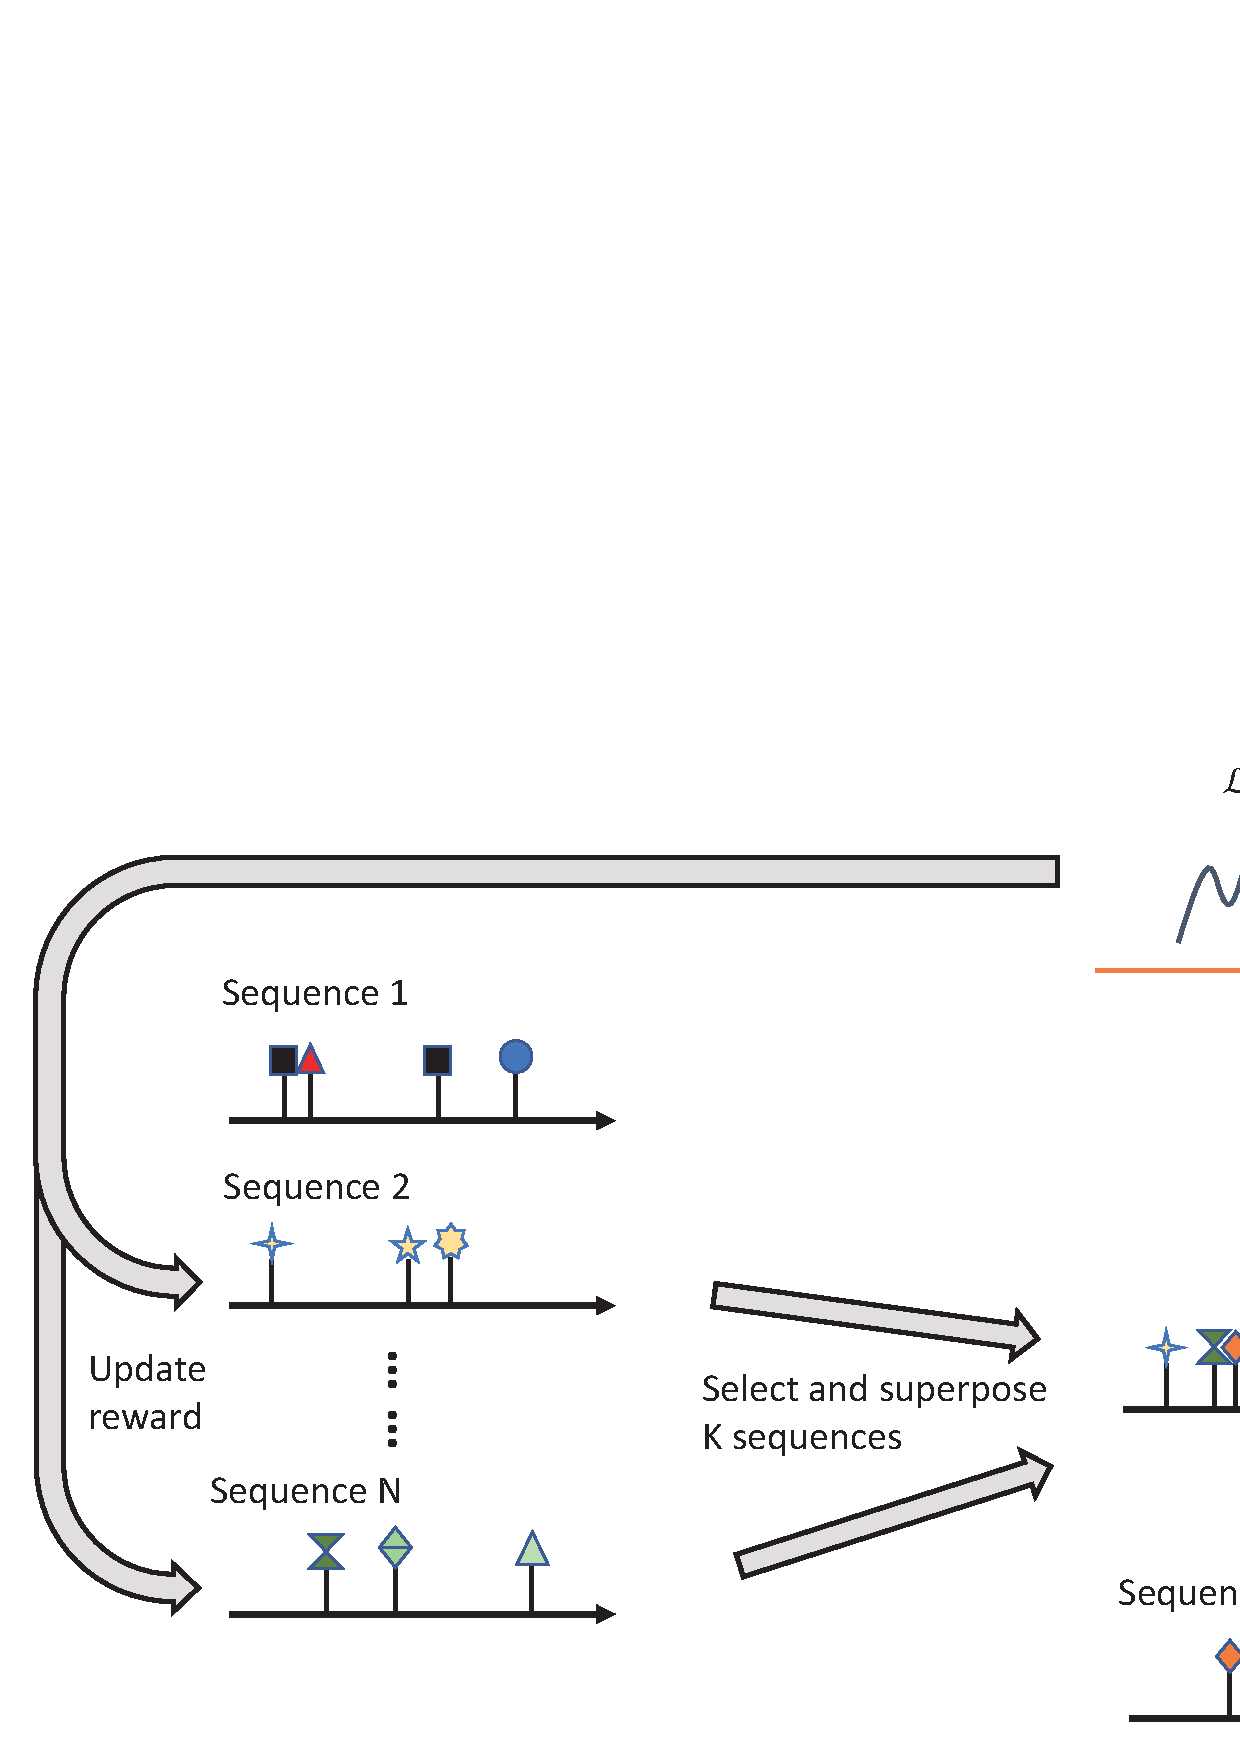
\includegraphics[width=0.9\linewidth]{figure1.pdf}}
\vspace{-10pt}
\caption{An illustration of the proposed self-organized Hawkes process model.}
\label{fig1}
\end{figure}

To address the problems above, we propose a self-organized Hawkes process (SOHP) model, which learns heterogeneous local Hawkes processes based on subsets of observed event sequences. 
The proposed model is motivated by a fact that the complex global interrelation between events tend to consist of simple local structures~\cite{lee2013local,lee2014local}. 
Thus, it is feasible to capture the triggering patterns in the complicated event sequences by many local Hawkes processes. 
In particular, Fig.~\ref{fig1} illustrates the principle of our model. 
We select and superpose $K$ sequences for each target sequence and learn a Hawkes process by maximum likelihood estimation (MLE) in an iterative way.
In each iteration, the $K$ sequences are selected based on a bandit algorithm, whose rewards are initialized by their optimal transport distance to the target sequence and updated according to the learned likelihood. 
Accordingly, the training sequences are organized adaptively as different subsets to support the learning of heterogeneous local Hawkes processes.\footnote{Here, ``heterogeneous'' means that both the event types of different Hawkes processes and the triggering patterns among the event types are different.}
In this inference phase, we merge the local Hawkes processes and make prediction of future events for each sequence.

This self-organization mechanism adjusts event sequences belonging to different Hawkes processes with training progress, which helps to capture diverse generative mechanisms of different target event sequences based on few observations. 
Additionally, for the local Hawkes processes, their numbers of event types are much smaller than the total number of the event types appearing in the whole set, which is beneficial for improving the scalability of Hawkes processes. 
We test our SOHP model in sequential recommendation tasks. 
Experimental results show that our model owns better capacity and interpretability, which achieves higher prediction precision than state-of-the-art methods.



% We make the event sequences belonging to each Hawkes process self-organized with the progress of training, which improve the capacity and interpretability of the model.


% Additionally, the work in~\cite{xu2018benefits} verified the improvement by the random strategy on selecting sequences. 
% Instead of purely random, however, we make the event sequences belonging to each Hawkes process self-organized with the progress of training, which improve the capacity and interpretability of the model.
% In addition, our model enhance the robustness to the data sparsity problem for the benefit from the superposition property of the Hawkes process \cite{xu2018benefits}.





\section{Proposed Model}
\subsection{Continuous-time recommendation based on Hawkes processes}

Denote $\{(t_i, c_i)\}_{i=1}^{I}$ as an event sequence, where the timestamp $t \in [0, T]$, event type $c\in\mathcal{C}$, and $(t_i, c_i)$ represents the $i$-th event with type $c_i$ and at time $t_i$. 
A temporal point process models the event sequence as a counting process $N = \{ N_c(t) | t \in [0, T], c\in\mathcal{C} \}$, where $N_c(t)$ is the number of type-$c$ events occurring till time $t$, and characterizes the expected instantaneous happening rate of the type-$c$ event at time $t$ by an intensity function: 
\begin{eqnarray}\label{eq:intensity}
\begin{aligned}
\lambda_c(t) := \frac{\mathbb{E}[\dd N_c(t)|\mathcal{H}_t^\mathcal{C}]}{\dd t},~\forall~c\in\mathcal{C}~\text{and}~t\in [0, T].
\end{aligned}    
\end{eqnarray}
where $\mathcal{H}_t^\mathcal{C}=\{(t_i, c_i)| t_i < t, c_i \in \mathcal{C}\}$ represents historical observations till time $t$.

As a special kind of temporal point process, Hawkes process is able to capture the triggering patterns among the event types in an explicit way. 
It formulates the intensity function above as
\begin{eqnarray}\label{eq:hp}
\begin{aligned}
\lambda_c(t) = \mu_c + \sideset{}{_{t_i < t}}\sum \phi_{cc_i} (t, t_i) = \mu_c + \sideset{}{_{t_i < t}}\sum a_{cc_i}\kappa(t- t_i),~\forall~c\in\mathcal{C},
\end{aligned}    
\end{eqnarray}
where $\mu_c$ represents the basic happening rate (a.k.a. base intensity) of the type-$c$ event. 
$\phi_{cc'} (t, t')$, $t'<t$ and $c,c'\in\mathcal{C}$, is called \textit{impact function}, which represents the influence of the type-$c'$ event at time $t'$ on the type-$c$ event at time $t$. 
Generally, the impact function $\phi_{cc'}$ is assumed to be shift-invariant and parameterized by $a_{cc'}\kappa(t -t')$, where $a_{cc'}\kappa(t)$ is a weighted decay function. 
For convenience, we can represent a Hawkes process as $\text{HP}(\bm{\mu},\bm{A})$, where $\bm{\mu}=[\mu_c]\in\mathbb{R}^{|\mathcal{C}|}$ represents the base intensity of the event types and $\bm{A}=[a_{cc'}]\in\mathbb{R}^{|\mathcal{C}|\times |\mathcal{C}|}$ is the infectivity matrix capturing the triggering patterns among the event types.


Hawkes process owns many useful properties. 
Firstly, the infectivity matrix corresponds to the adjacency matrix of the \textit{Granger causality graph} of event types~\cite{xu2016learning}, which represents the self- and mutually-triggering patterns hidden in event sequences explicitly. 
Secondly, the \textit{superposition property} of Hawkes process~\cite{xu2018benefits} shows that when learning a Hawkes process from event sequences, we can superpose observed event sequences to obtain an event sequence with much denser events and learn the Hawkes process with a tighter bound of excess risk~\cite{xu2018benefits}, which improves the robustness to the data sparsity problem.

Given a set of event sequences $\mathcal{N}=\{N^u\}_{u\in\mathcal{U}}$, we can learn the Hawkes process by the maximum likelihood estimation (MLE):
\begin{eqnarray}\label{eq:mle}
\begin{aligned}
\sideset{}{_{\bm{\theta}}}\min -\log \mathcal{L}(\mathcal{N};\bm{\theta}) + \gamma \mathcal{R}(\bm{\theta}), 
\end{aligned}    
\end{eqnarray}
where $\bm{\theta}=\{\bm{\mu},\bm{A}\}$ represents the model parameter, $\mathcal{L}(\mathcal{N};\bm{\theta})$ is the likelihood function of the event sequences~\cite{daley2008introduction}:
\begin{eqnarray}\label{eq:likelihood}
\begin{aligned}
\mathcal{L}(\mathcal{N};\lambda) = \sideset{}{_{u\in\mathcal{U}}}\prod \Bigl(\sideset{}{_{(c_i^u, t_i^u) \in N^u}}\prod \lambda_{c_i^u}(t_i^u) \times \exp \bigl( - \sideset{}{_{c\in\mathcal{C}}}\sum\sideset{}{_{0}^T}\int \lambda_c^u(s) \dd s \bigr)\Bigr),
\end{aligned}    
\end{eqnarray}
and $\mathcal{R}(\cdot)$ represents the regularization term imposed on the model parameters, such as the sparsity and the low-rank regularizers on $\bm{A}$~\cite{zhou2013learning}.
This method applies the idea that the observed events are most probable and updates parameters to maximize the likelihood of the observed events. 

After the intensity function is obtained, we could predict the type of next event in the future. 
In particular, given the history till time $t$ ($i.e.$, $\mathcal{H}_t^{\mathcal{C}}$), the probability of the type-$c$ event at $t + \Delta t$ could be computed by~\cite{xu2016patient}:
\begin{eqnarray}\label{eq:prediction}
\begin{aligned}
p(c | t+\Delta t, \mathcal{H}_t^{\mathcal{C}}) = \frac{\lambda_c(t+\Delta t)}{\sum_{c'\in\mathcal{C}}\lambda_{c'} (t+\Delta t)}.
\end{aligned}    
\end{eqnarray}

The Hawkes process above has the potentials to capture purchasing behaviors of the users at the e-commercial platform and construct a sequential recommendation system in the continuous-time domain~\cite{xu2018benefits}.
In such a situation, the event sequences correspond to the purchasing behaviors of different users and the event types correspond to different items. 
By learning a Hawkes process, we model the expected instantaneous purchasing rate of the users over time, where the infectivity matrix $\bm{A}$ reflects the triggering patterns among the items and the base intensity $\bm{\mu}$ reflects the intrinsic popularity of the items.

However, on one hand, the real-world behaviors of the users may yield different generative mechanisms, which correspond to different Hawkes processes. 
On the other hand, the purchasing behaviors of each individual are often very sparse, which are insufficient to learn a Hawkes process model. 
To overcome this conflict, we propose the self-organized Hawkes process model below, learning multiple local Hawkes processes robustly by organizing the event sequences of different users in an adaptive way.


\subsection{Self-organized Hawkes processes}
As aforementioned, the proposed self-organized Hawkes process model is motivated by the work in~\cite{lee2013local,lee2014local}, which captures the complicated global relations among all the items by learning and merging simple local relations among subsets of items.
Therefore, in our SOHP model, each event sequence corresponds to a local Hawkes process. 

The key challenge is how to solve the data sparsity problem --- in the training phase, we need to suppress the risk of over-fitting caused by insufficient training events, while in the inference phase, we need to explore a sufficient large item space, predicting the items that may never appear in the sequence. 
Fortunately, the superposition property of Hawkes process helps us to build an algorithmic framework that is robust to this challenge above.
\begin{theorem}[Superposition Property~\cite{xu2018benefits}]\label{them:superpose}
For a set of independent Hawkes processes with a shared infectivity matrix, $i.e.$, $\{N^u \sim \text{HP}(\bm{\mu}^u,\bm{A})\}_{u\in\mathcal{U}}$, the superposition of their sequences satisfies $\sum_{u\in\mathcal{U}} N^u \sim \text{HP}(\sum_{u\in\mathcal{U}} \bm{\mu}^u,\bm{A})$.  
\end{theorem}
With the help of this property, we can superpose sparse event sequences randomly and learn the infectivity matrix with much denser training events. 
The work in~\cite{xu2018benefits} demonstrates that this superposition-based strategy helps us to achieve a tighter bound of excess risk in the learning phase.

However, when learning multiple heterogeneous Hawkes processes in a complicated scenario, the event sequences belong to different Hawkes processes that have various infectivity matrices. 
In such a situation, superposing the event sequences randomly is likely to disobey the assumption imposed in Theorem~\ref{them:superpose} ($i.e.$, the Hawkes processes have the same infectivity matrix). 
\textbf{To overcome this problem, we design a new self-organization mechanism, selecting event sequences for each local Hawkes process and adjusting the selection with the training progress.}
Mathematically, denote $\mathcal{N} = \{N^u\}_{u \in \mathcal{U}}$ as a set of real-world event sequences. 
Our learning task becomes
\begin{eqnarray}\label{eq:task}
\begin{aligned}
\sideset{}{_{\{\bm{\theta}^u\}_{u\in\mathcal{U}}}}\min  \sideset{}{_{\mathcal{N}^u \subset \mathcal{N}}}\min
-\sideset{}{_{u \in \mathcal{U}}}\sum\frac{1}{|N^u \cup \mathcal{N}^u|}\log \mathcal{L}(N^u \cup \mathcal{N}^u; \bm{\theta}^u),
\end{aligned}    
\end{eqnarray}
where $\mathcal{N}^u=\{N^{s_1};\ldots;N^{s_K}\}$ represents the $K$ neighbors of the $u$-th sequence. 
$N^u \cup \mathcal{N}^u$ constructs a subset of event sequences for learning the $u$-th local Hawkes processes.
Here, we aim at optimizing the parameters of the Hawkes processes $\{\bm{\theta}^u\}_{u\in\mathcal{U}}$ and the selection of their training sets jointly.

\section{Learning Algorithm}
\subsection{A reward-augmented bandit algorithm}
The learning problem in (\ref{eq:task}) is NP-hard. 
Therefore, we propose a novel reward-augmented bandit algorithm to solve it heuristically. 
Intuitively, we hope that 1) the selected sequences are similar to the target sequence; 2) the selected sequences own some randomness to avoid the over-fitting problem. 
To achieve this aim, for each target sequence, we treat the selection of its neighbors ($i.e.$, the training set of a Hawkes process) as a multi-armed bandit problem~\cite{auer2002nonstochastic}, selecting their neighbors according to the potential \textit{rewards}. 
The accumulation of the rewards formulates a benefit matrix $\bm{B}=[b_{u,k}]\in\mathbb{R}^{|\mathcal{U}|\times |\mathcal{U}|}$, where $b_{u,k}$ represents the benefit from selecting the $k$-th sequence for the $u$-th Hawkes process. 

The key of our algorithm is the design and the update of the benefit matrix. 
Initially, we define the initial benefit based on the optimal transport distance between event sequences~\cite{xu2021hawkes}. 
This distance is applicable to the sequences with heterogeneous event types. 
Specifically, for $N^u=\{N_i^u \}_{i \in \mathcal{C}_u}$ and $N^v=\{N_j^v\}_{j \in \mathcal{C}_v}$, where $\mathcal{C}_u$ and $\mathcal{C}_v$ are respectively the sets of event types appearing in $N^u$ and $N^v$, and $N_i^u$ is the counting process associated with the $i$-th event types in $N^u$. 
Then, the optimal transport distance between $N^u$ and $N^v$ is defined as
\begin{eqnarray}\label{eq:ot}
\begin{aligned}
d(N^u, N^v) 
& := \sideset{}{_{\bm{T} \in \Pi (\frac{1}{|\mathcal{C}_u|} \bm{1}_{|\mathcal{C}_u|}, \frac{1}{|\mathcal{C}_v|} \bm{1}_{|\mathcal{C}_v|})}}\min \sideset{}{_{i \in \mathcal{C}_u, j \in \mathcal{C}_v}}\sum T_{ij} d(N_i^u, N_j^v)\\
&= \sideset{}{_{\bm{T} \in \Pi (\frac{1}{|\mathcal{C}_u|} \bm{1}_{|\mathcal{C}_u|}, \frac{1}{|\mathcal{C}_v|} \bm{1}_{|\mathcal{C}_v|})}}\min \langle \bm{D}_{uv}, \bm{T} \rangle
\end{aligned}    
\end{eqnarray}
where $\Pi (\frac{1}{|\mathcal{C}_u|} \bm{1}_{|\mathcal{C}_u|}, \frac{1}{|\mathcal{C}_v|} \bm{1}_{|\mathcal{C}_v|})=\{\bm{T}\geq \bm{0}|\bm{T}\bm{1}=\frac{1}{|\mathcal{C}_u|} \bm{1}_{|\mathcal{C}_u|}, \bm{T}^{\top}\bm{1}=\frac{1}{|\mathcal{C}_v|} \bm{1}_{|\mathcal{C}_v|}\}$ represents the set of joint distributions with marginals $\frac{1}{|\mathcal{C}_u|} \bm{1}_{|\mathcal{C}_u|}$ and $\frac{1}{|\mathcal{C}_v|} \bm{1}_{|\mathcal{C}_v|}$. 
$\bm{D}_{uv}=[d(N_i^u, N_j^v)] \in \mathbb{R}^{|\mathcal{C}_u| \times |\mathcal{C}_v| }$ is a distance matrix, where $d(N_i^u, N_j^v) = \frac{1}{T} \int_0^T|N_i^u(t) - N_j^v(t)| \dd t$ represents the discrepancy between the sequence of the type-$i$ events and that of the type-$j$ events.
The matrix $\bm{T}=[T_{ij}]$ that minimizes (\ref{eq:ot}) is called the optimal transport matrix. 
Fig.~\ref{fig2} illustrates the optimal transport distance.
The optimal transport distance can be calculated efficiently by the Sinkhorn scaling algorithm~\cite{cuturi2013sinkhorn}.

\begin{figure}[t]
\centerline{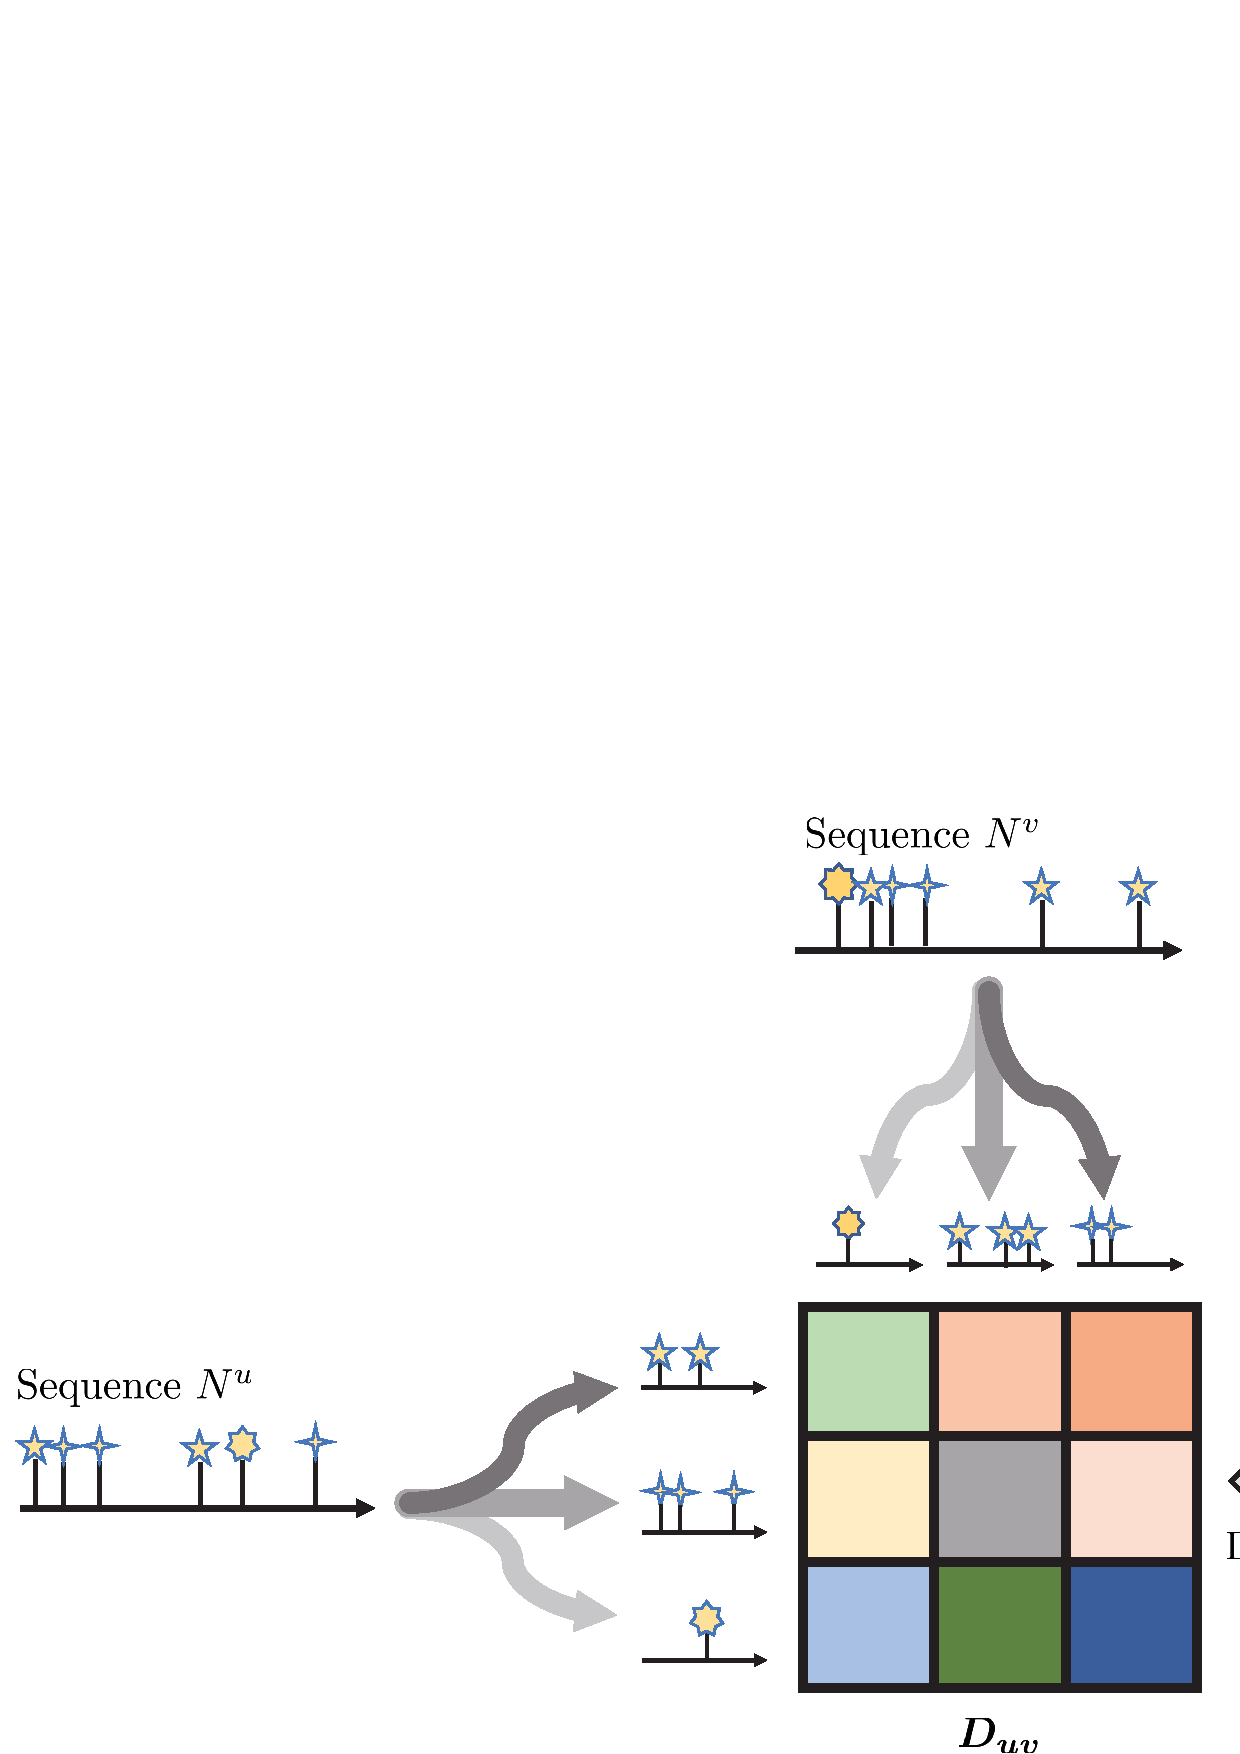
\includegraphics[width=0.7\linewidth]{figure2.pdf}}
\vspace{-10pt}
\caption{The optimal transport distance between heterogeneous event sequences.}
\label{fig2}
\end{figure}

\begin{algorithm}[t]
\caption{Learning SOHP via a reward-augmented bandit algorithm}\label{alg1}
\hspace*{0.02in} {\bf Input:}
Event sequences $\mathcal{N}=\{N^u\}_{u \in \mathcal{U}}$, distance matrix of sequences $\bm{D}=[d(N^u, N^v)] \in \mathbb{R}^{|\mathcal{U}| \times |\mathcal{U}|}$, the number of iterations $L$, the number of neighbors $K$, learning rate $\alpha$\\
\hspace*{0.02in} {\bf Output:} 
benefit matrix $\bm{B}\in \mathbb{R}^{|\mathcal{U}| \times |\mathcal{U}|}$ and model parameters $\{\bm{\theta}^u\}_{u\in\mathcal{U}}$.
\begin{algorithmic}[1]
\For{$u = 1:|\mathcal{U}|$} 
    \State Initialize $b_{u,k}=\max_{v}d(N^u, N^v) - d(N^u, N^k)$ for $k \in\mathcal{U}$.
    \For{$l=1:L$}
        \If{$l<L$}
        \State Set $\bm{p}=[\frac{b_{u,1}}{\sum_i b_{u,i}},..,\frac{b_{u,|\mathcal{U}|}}{\sum_i b_{u,i}} ]$, sample $\{N^{s_1},..,N^{s_K}\}$ from $\mathcal{N}$ with $\bm{p}$.
        \Else 
        \State Select $\{N^{s_1},..,N^{s_K}\}$ with the $K$ highest benefits.
        \EndIf
        \State Learn the model parameter $\bm{\theta}^u$ from $ \{N^u\} \cup \{N^{s_1},..,N^{s_K}\}$ by (\ref{eq:mle}).
        \For{$k=s_1:s_K$}
        \State $b_{u,k} = b_{u,k} + \alpha \mathcal{L}(N^{s_k};\bm{\theta}^u)$
        \EndFor
    \EndFor
\EndFor
\end{algorithmic}
\end{algorithm}

Accordingly, we initialize the benefit $b_{u,k}$ as $\max_{v}d(N^u, N^v) - d(N^u, N^k)$.
In the training phase, we treat the normalized benefits as the probabilities of the sequences and select them accordingly.
Then, we regard the likelihood of selected event sequences in each iteration as the intermediate reward and update the corresponding benefit by accumulating the reward accordingly. 
In the end of iteration, we select $K$ sequences with the highest benefits for each sequence $N^u$.\footnote{We tried more sophisticated bandit algorithm like the Upper Confidence Bound (UCB) method~\cite{audibert2009exploration} to select the sequences, but our experimental results show that the proposed greedy algorithm achieves the best performance.}   
The steps of our reward-augmented bandit algorithm are shown in Algorithm~\ref{alg1}. 
It should be noted that this algorithm reduces the computational complexity of learning Hawkes process: in each iteration, we only learn each Hawkes process based on the superposition of $K$ sequences, which greatly reduced the number of event types for each Hawkes process.

\subsection{Merging learned Hawkes processes}

% In Algorithm~\ref{alg2}, with the benefit matrix $\bm{B}$ obtained in Algorithm~\ref{alg1}, we select $K$ sequences $\{N^{s_1};\ldots;N^{s_K}\}$ of the most similar ones and superpose them for each sequence $N$, respectively.\footnote{We tried more sophisticated bandit algorithm like the Upper Confidence Bound (UCB) method~\cite{audibert2009exploration} to select the sequences, but our experimental results show that the proposed greedy algorithm achieves the best performance.}  
In the inference phase, instead of leveraging the intensity function of each local Hawkes process to make predictions, we first merge the learned infectivity matrices by superposition operations, as shown in Fig.~\ref{fig3}. 
Then, for each sequence, we predict its future events based on its local base intensity and the global infectivity matrix.
Note that in the sequential recommendation scenario this inference strategy achieves an exploration–exploitation trade-off: the local base intensity reveals the preference of the user on purchased items while using the global infectivity matrix helps the system to explore the items that she never saw but might be interested in.



\begin{figure}[t]
\centerline{\includegraphics[width=0.7\linewidth]{figure3.pdf}}
\vspace{-10pt}
\caption{An illustration of merging local infectivity matrices. The purple ones correspond to the overlapped event types, whose values are accumulated together.}
\label{fig3}
\end{figure}


\section{Related Work}
\textbf{Sequential recommendation}
By modeling the sequential behaviors from user historical records, sequential recommendation predicts future interests and recommend items. Besides the shopping recommendation, sequential recommendation has also been widely used in various application scenarios, such as web recommendation~\cite{zhang2015task}, music recommendation~\cite{chen2012playlist}, and Point-of-Interest recommendation~\cite{cheng2013you,feng2015personalized}, etc.
These years, many cutting-edge techniques have been applied into the sequential recommend, $e.g.$, FPMC~\cite{rendle2010factorizing} integrated matrix factorization and Markov chains, HRM~\cite{wang2015learning} regarded representation learning as latent factors, they modeled the sequential behavior patterns via every two contiguous historical records. 
DREAM~\cite{yu2016dynamic} is based on recurrent neural network (RNN) and learns the global sequential behavior patterns.
These models all captured the contiguous behavior information without taking time interval between them into considering. Instead, we leverage the time stamps of every behavior to calculate efficiently the mutual effect of them, achieving continuous-time recommendation.


\textbf{Hawkes process}
Because of its effectiveness on modeling the triggering patterns among real-world events, Hawkes process has been widely used in many scenarios, such as high frequency finance \cite{bacry2015hawkes}, and fake news mitigation \cite{farajtabar2017fake}. 
Meanwhile, many variants of Hawkes process have been researched and developed, such as the Hawkes process with self-attention mechanisms~\cite{zhang2019self,zuo2020transformer}. 
Recently, the superposition of Hawkes process has been verified to be effective in both theory and experiments~\cite{xu2018benefits}. 
The model applied a random algorithm to select sequences and learned a single Hawkes process.
Our work, however, demonstrate that making superposition with the help of a bandit algorithm is more valid for learning multiple Hawkes processes.

\textbf{Multi-armed bandit problem}
The multi-armed bandit problem denotes a problem where we need to make choices to maximize expected gain under some constraints~\cite{robbins1952some}. 
These years, many bandit algorithms have been proposed, such as the Upper Confidence Bounds algorithm~\cite{li2010contextual,chu2011contextual,bouneffouf2019optimal}, adaptive epsilon-greedy strategy based on Bayesian ensembles~\cite{gimelfarb2020epsilon}, and behavior constrained Thompson Sampling~\cite{balakrishnan2019incorporating}, etc.
In this paper, we make an attempt to apply the bandit algorithm to select training sequences for Hawkes processes.


\section{Experiments}
\subsection{Implementation details}
We experiment on the Amazon review dataset~\cite{mcauley2015image}. 
This dataset contains product reviews from Amazon spanning May 1996 - July 2014. 
We select five product categories as our datasets to evaluate our model, including ``Instant Video'', ``Musical Instruments'', ``Video Games'', ``Baby'' and ``Patio, Lawn and Garden''.
To be specific, we preprocess the datasets as follows.
We select those items with more than 40 reviews. Then, their users need to satisfy three conditions: (i) the ratings they gave to these items are bigger than 4; (ii) there are at most 3 reviews spanning January 2014 - April 2014; (iii) there are at least 1 review from April 2014 to July 2014.
The statistics of the final datasets are shown in Table~\ref{tab1}.
After learning the behaviors of users from January 2014 to April 2014, our model predicts items for them from April 2014 to July 2014.

\begin{table}[t]
\centering
\caption{Statistics of our datasets}
    \begin{tabular}{c|c|c|c|c|c}
    \hline
    \hline
    Categories 
    & Musical Instruments 
    & Baby
    & Video Games
    & Garden
    & Instant Video\\
    \hline
    \#Users 
    & 471
    & 1979
    & 2142
    & 1812
    & 5948\\
    \#Items 
    & 678
    & 2134
    & 2104
    & 2064
    & 1344\\
    \#Ratings 
    & 1218
    & 6070
    & 6126
    & 4976
    & 15470\\
    \hline\hline
    \end{tabular}%
\label{tab1}%
\end{table}%

To demonstrate the superiority of our SOHP model, we adopt the following state-of-the-art methods as baselines for comparisons. 
\textbf{SVD}: Singular value decomposition, a classical method from linear algebra is getting popular in recommender systems; 
\textbf{kNN}: user-based K-nearest neighbors algorithm, a non-parametric classification and regression method; 
\textbf{BPR}: Bayesian personalized ranking~\cite{rendle2012bpr}, a popular method for top-N ranking recommendation; 
\textbf{SLIM}: Sparse linear method~\cite{ning2011slim}, a simple and effective method for top-N recommendation; 
\textbf{FPMC}: Factorized personalized Markov chains~\cite{rendle2010factorizing}, one of the stat-of-the-art models for sequential recommendation based on matrix factorization and Markov chains. Each item is regarded as a basket in this model.
\textbf{SHP}: The superposed Hawkes process~\cite{xu2018benefits} that learn a single Hawkes process by randomly superpose event sequences. 
For each model, denote the top-N recommended items for user $u$ as $R^u = \{r_1^u,\ldots,r_N^u \}$, where $r_i^u$ is ranked at the $i$-th position, and the set of real purchased items $T^u$, respectively.
We use the top-N precision, recall and F1 score as the measurements.
% \begin{eqnarray*}
% \begin{aligned}
% P@N &= \frac{1}{|\mathcal{U}|}\sum_u P_u@N = \frac{1}{|\mathcal{U}|} \sum_u \frac{|R_u \cap T_u|}{|R_u|}\\
% R@N &= \frac{1}{|\mathcal{U}|}\sum_u R_u@N = \frac{1}{|\mathcal{U}|} \sum_u \frac{|R_u \cap T_u|}{|T_u|}\\
% F_1@N &= \frac{1}{|\mathcal{U}|}\sum_u F_{1u}@N = \frac{1}{|\mathcal{U}|} \sum_u \frac{2 \cdot P_u@N \cdot R_u@N}{P_u@N + R_u@N}
% \end{aligned}    
% \end{eqnarray*}

When implementing our method, the number of iterations $L$ for each user is set as $20$ and the learning rate $\alpha$ is set as $0.1$. 
We primarily set the number of neighbor event sequences $K=10$, and the effect of setting different $K$ is studied in the experiments.
When learning the superposition of Hawkes processes, we empirically set the decay function $\kappa(t)$ as $\exp(-\beta t)$, where $\beta=3e-4$, and use no regularization term.
For each user, $10$ items are recommended.



\subsection{Comparisons and analysis}
Table~\ref{tab2} summarizes the performance for the baselines and our method on the five datasets. 
For all the datasets except ``Instant Video'', our SOHP model achieves better performance than its competitors. 
Specifically, in the category ``Musical instrument'', the result of our model is $13\%$ higher than that of the best baseline ($i.e.$, FPMC), and the difference would be up to $48\%$ by tuning $K$ in the subsequent experiments. 
The results indicate the effectiveness of our model for sequential recommendation.


Essentially, for the users, the more neighbor event sequences are considered, the more intersections their training sets have. 
Accordingly the local Hawkes processes learned based on the sets may more similar. 
In such a situation, our SOHP model may tend to recommend different users similar items.
We are curious about whether and how the number of neighbors affects the recommendation results.
To do so, we study the performance of our model on F1@10
by tuning $K$ in the range of $\{2,5,10,20,50,100\}$. 
Results are shown in Fig.~\ref{fig4}. 

For the categoies ``Musical Instruments'' and ``Baby'', as the increase of $K$, the performance of them gets better. 
At this moment, the model learns more popular interests and will be more inclined to recommend the most popular items. 
For the category ``Musical Instrument'', the users tend to focus on a limited number of items and purchase similar ones.
In the case of the category ``Baby'', babies cannot comment on the items, so parents often choose the most popular products.


\begin{table}[t]
    \centering
    \caption{Summary of the performance for baselines and our model}
    \resizebox{.99\columnwidth}{!}{
      \begin{tabular}{c|ccc|ccc|ccc|ccc|ccc}
      \hline
      Datasets & \multicolumn{3}{c|}{Musical Instruments} & \multicolumn{3}{c|}{Baby} & \multicolumn{3}{c|}{Video Games} & \multicolumn{3}{c|}{Garden} & \multicolumn{3}{c}{Instant Video} \\
      \hline
      \hline
      Measures@10(\%) & P     & R     & F1    & P     & R     & F1    & P     & R     & F1    & P     & R     & F1    & P     & R     & F1 \\
      \hline
      SVD   & 0.106 & 1.061 & 0.193 & 0.121 & 0.735 & 0.207 & 0.065 & 0.498 & 0.113 & 0.055 & 0.395 & 0.094 & 0.126 & 1.052 & 0.221 \\
      kNN   & 0.382 & 2.671 & 0.649 & 0.389 & 2.513 & 0.638 & 0.661 & 4.915 & 1.163 & 0.237 & 1.751 & 0.405 & 0.817 & 6.901 & 1.435 \\
      BPR   & 0.467 & 3.750 & 0.811 & 0.389 & 2.469 & 0.635 & 0.658 & 4.864 & 1.112 & 0.110 & 0.762 & 0.185 & 0.859 & 7.049 & 1.503 \\
      SLIM  & 0.212 & 1.351 & 0.347 & 0.111 & 0.712 & 0.180 & 0.499 & 3.595 & 0.835 & 0.242 & 1.544 & 0.401 & \textbf{1.333} & \textbf{11.428} & \textbf{2.351} \\
      FPMC  & 0.594 & 4.193 & 1.006 & 0.283 & 1.912 & 0.470 & 0.556 & 3.799 & 0.927 & 0.171 & 1.117 & 0.285 & 0.931 & 7.413 & 1.622 \\
      SHP & 0.361 & 2.406 & 0.604 & 0.258 & 1.734 & 0.432 & 0.317 & 2.037 & 0.525 & 0.199 & 1.350 & 0.331 & 0.933 & 7.406 & 1.623 \\
      Our methods & \textbf{0.658} & \textbf{5.149} & \textbf{1.138} & \textbf{0.389} & \textbf{2.640} & \textbf{0.651} & \textbf{0.700} & \textbf{5.108} & \textbf{1.180} & \textbf{0.248} & \textbf{1.801} & \textbf{0.436} & 0.999 & 7.911 & 1.738 \\
      \hline
      \hline
      \end{tabular}%
    }
    \label{tab2}%
  \end{table}%
  
\begin{figure}[t]
\centerline{\includegraphics[width=0.95\linewidth]{figure4.png}}
\vspace{-10pt}
\caption{Performance of our model under different number of neighbors $K$. }
\label{fig4}
\end{figure}

For the categories ``Video Games'' and ``Garden'', the performance becomes the best at $K \  \approx \ 10 $ and degrades a lot when further increasing neighbors. 
A potential reason for this phenomenon is that the purchasing behaviors in these two categories have diverse patterns. 
As aforementioned, when there are too many neighbors, our model will tend to recommend the most popular items to all the users, which is unsuitable for these two categories.

For the category ``Instant Video'', however, we find that our model is inferior to the SLIM method, and the performance is stable with respect to the number of neighbors. 
According to our analysis, a possible reason for this phenomenon is that for most users, their choice of instant video tend to be influenced by Amazon's recommendations or the most popular video list, which may not be suitable for sequential recommendation. 
Evidence supporting this explanation is that the FPMC, which is also a sequential recommendation model, has poor performance as well for this category.



\section{Conclusion}
In this paper, we proposed a framework combining bandit algorithm with Hawkes processes, which provides a new way to learn complicated sequential models robustly from insufficient observations. 
We designed the reward of the Bandit algorithm, and exerted the greedy strategy to update the reward iteratively. 
The proposed model achieved encouraging performance on continuous-time sequential recommendation.
In the future, we plan to design new formulation of rewards and update rewards by more efficient strategies. 
Additionally, we will make attempts to set the number of neighbor event sequences adaptively to further improve our model.

\bibliographystyle{splncs04}
\bibliography{references}

\clearpage
\newpage



\end{document}
